\documentclass[aspectratio=169,10pt]{beamer}

\usetheme{Madrid}

% OpenFaaS Brand Colors (Deep Navy and Bright Piercing Blue)
\definecolor{OpenFaaSDark}{RGB}{9, 30, 54}
\definecolor{OpenFaaSLight}{RGB}{0, 146, 210}

% --- Additional System Colors (Aligned with your theme) ---
\definecolor{ComputeColor}{RGB}{66,133,244}     % Blue (functions)
\definecolor{StorageColor}{RGB}{52,168,83}      % Green (S3)
\definecolor{QueueColor}{RGB}{251,188,5}        % Yellow (SQS)
\definecolor{AWSColor}{RGB}{255,153,0}          % AWS Orange
\definecolor{UserColor}{RGB}{120,120,120}       % Neutral

\setbeamercolor{palette primary}{bg=OpenFaaSLight, fg=white}
\setbeamercolor{palette secondary}{bg=OpenFaaSLight!80!black, fg=white}
\setbeamercolor{palette tertiary}{bg=OpenFaaSDark, fg=white}
\setbeamercolor{palette quaternary}{bg=black, fg=white}

\setbeamercolor{title}{bg=OpenFaaSDark, fg=white}
\setbeamercolor{titlelike}{bg=OpenFaaSDark, fg=white}
\setbeamercolor{frametitle}{bg=OpenFaaSDark, fg=white}
\setbeamercolor{structure}{fg=OpenFaaSLight}
\setbeamercolor{item}{fg=OpenFaaSLight}

\setbeamertemplate{blocks}[rounded][shadow=true]
\setbeamertemplate{caption}[numbered]
\setbeamercolor{block title}{bg=OpenFaaSLight, fg=white}
\setbeamercolor{block body}{bg=OpenFaaSLight!10, fg=black}
\setbeamercolor{block title alerted}{bg=red!80!black, fg=white}
\setbeamercolor{block body alerted}{bg=red!10, fg=black}
\setbeamercolor{block title example}{bg=OpenFaaSDark, fg=white}
\setbeamercolor{block body example}{bg=OpenFaaSDark!10, fg=black}

\usepackage{booktabs}
\usepackage{graphicx}
\usepackage{hyperref}
\usepackage{tikz}
\usetikzlibrary{shapes.geometric, arrows.meta, positioning, calc, fit, backgrounds}
\usepackage{pgfplots}
\usepackage{adjustbox}
\pgfplotsset{compat=1.18}

% --- TikZ Styles (consistent across slides) ---
\tikzset{
    base/.style={
        draw,
        rounded corners=3pt,
        minimum width=3.2cm,
        minimum height=1.2cm,
        text width=3cm,
        align=center,
        font=\small,
        inner sep=4pt
    },
    user/.style={base, fill=UserColor!20},
    gateway/.style={base, fill=OpenFaaSLight!20, draw=OpenFaaSLight, thick},
    compute/.style={base, fill=ComputeColor!20, draw=ComputeColor, thick},
    storage/.style={base, fill=StorageColor!20, draw=StorageColor, thick},
    queue/.style={base, fill=QueueColor!20, draw=QueueColor, thick},
    aws/.style={base, fill=AWSColor!20, draw=AWSColor, thick},
    arrow/.style={->, thick, draw=OpenFaaSDark}
}

\title{VideoSearcher Serverless Pipeline using OpenFaaS}
\subtitle{Load Testing \& Performance Evaluation}
\author{Soumyadeep Sharma}
\date{\today}

\begin{document}

\begin{frame}[plain]
    \titlepage
\end{frame}

\begin{frame}{Introduction to OpenFaaS}
    \begin{columns}
        \begin{column}{0.48\textwidth}
            \begin{block}{What is OpenFaaS}
                \textbf{OpenFaaS (Function as a Service)} is an open-source framework for deploying serverless functions and microservices to \textbf{Kubernetes or Docker Swarm}. It enables developers to package any code, binary, or container image into a portable, auto-scaling function that responds to events.
            \end{block}
        \end{column}
        \begin{column}{0.52\textwidth}
            \begin{figure}
                \centering

                \begin{adjustbox}{max size={\textwidth}{0.65\textheight}}
                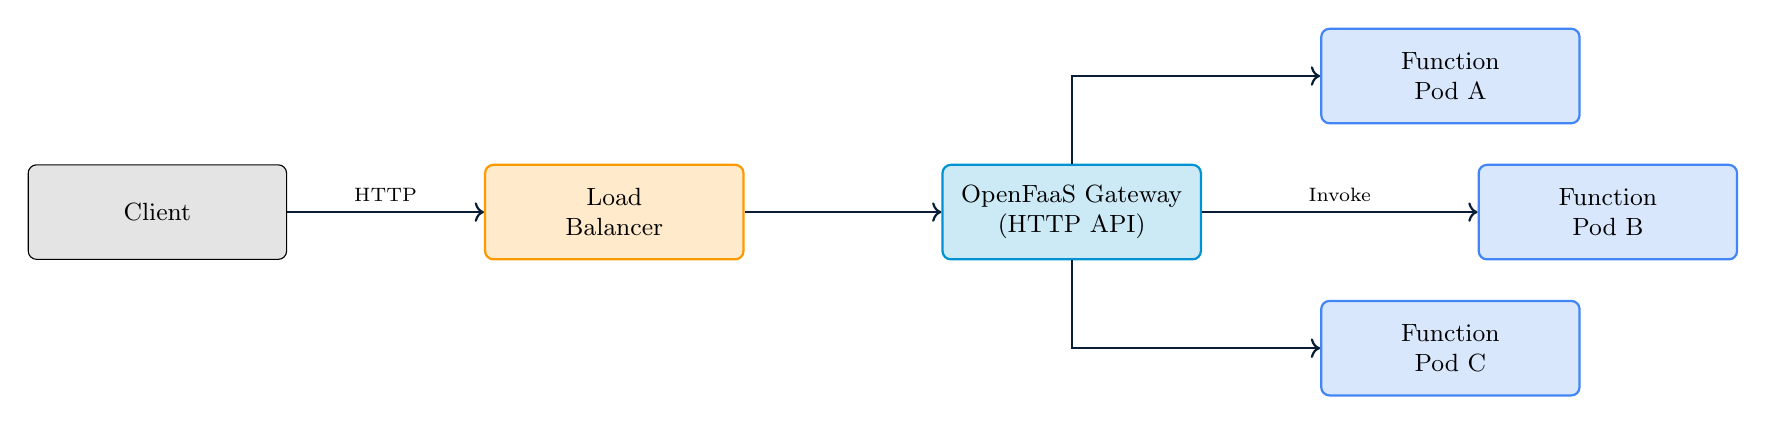
\begin{tikzpicture}[node distance=2.5cm]

                    \node<1->[user] (user) {Client};
                    \node<2->[aws, right=of user] (lb) {Load\\Balancer};
                    \node<3->[gateway, right=of lb] (gateway) {OpenFaaS Gateway\\(HTTP API)};
                    
                    \node<4->[compute, above right=0.5cm and 1.5cm of gateway] (fn1) {Function\\Pod A};
                    \node<4->[compute, right=of gateway, xshift=1cm] (fn2) {Function\\Pod B};
                    \node<4->[compute, below right=0.5cm and 1.5cm of gateway] (fn3) {Function\\Pod C};
                    
                    \draw<2->[arrow] (user) -- node[midway, above, font=\scriptsize] {HTTP} (lb);
                    \draw<3->[arrow] (lb) -- (gateway);
                    \draw<4->[arrow] (gateway) -- node[midway, above, font=\scriptsize] {Invoke} (fn2);
                    \draw<4->[arrow] (gateway) |- (fn1);
                    \draw<4->[arrow] (gateway) |- (fn3);
                
                \end{tikzpicture}
                \end{adjustbox}
                
                \caption{High-Level OpenFaaS HTTP API Flow Architecture.}
            \end{figure}
        \end{column}
    \end{columns}
\end{frame}

\begin{frame}{Introduction to OpenFaaS (cont.)}
        \begin{block}{Some Key Capabilities of OpenFaaS}
                \begin{itemize}[<+->]
                    \item \textbf{Package Anything:} Any container or script can become a serverless API.
                    \item \textbf{Event-Driven:} Seamlessly connects with message queues like AWS SQS and NATS.
                    \item \textbf{No Vendor Lock-in:} Deploy functions locally or on any cloud without changing code logic.
                    \item \textbf{Auto-Scaling:} Functions automatically scale up or down based on incoming requests, including scale-to-zero.
                    \item \textbf{Language Agnostic:} Supports multiple programming languages through templates (Python, Node.js, Go, etc.).
                    \item \textbf{Kubernetes-Native:} Runs seamlessly on Kubernetes for orchestration, networking, and scaling.
                    \item \textbf{Container-Based:} Uses Docker containers to package and run functions consistently across environments.
                    \item \textbf{Easy CI/CD Integration:} Works with popular pipelines for automated build and deployment.
                    \item \textbf{Built-in Monitoring:} Integrates with Prometheus for metrics, logging, and performance tracking.
                \end{itemize}
            \end{block}
\end{frame}
\begin{frame}{Project Goal}
    \begin{block}{What I Set Out to Do}
        \begin{itemize}[<+->]
            \item The main goal of my project was to take the VideoSearcher pipeline and deploy it as serverless functions using OpenFaaS.
            \item I wanted the system to run reliably on the cloud using AWS EKS, while still being testable locally.
            \item One strict constraint I followed was that I did not modify any of the original \texttt{main.py} files.
            \item So instead of changing the code, I designed the entire infrastructure around it to make it cloud-compatible.
        \end{itemize}
    \end{block}
\end{frame}
\begin{frame}{Project Overview}
    \begin{block}{Understanding the Problem}
        \begin{itemize}[<+->]
            \item The project is essentially a multi-stage video processing pipeline, where each stage is a standalone Python script.
            \item These scripts follow a simple CLI pattern, taking input and output paths as arguments.
            \item One of the biggest challenges I faced was that the code depends on a package called \texttt{aisprint}, which is not publicly available.
            \item So I had to find a way to make everything run smoothly without modifying or breaking the original implementation.
        \end{itemize}
    \end{block}
\end{frame}
\begin{frame}{Pipeline Stages}
    \begin{block}{How the Pipeline Works}
        \begin{itemize}[<+->]
            \item The pipeline processes a video step-by-step:
            \begin{itemize}[<+->]
                \item First, it splits the audio and video streams
                \item Then it detects speech segments
                \item Based on those timestamps, it cuts the video into clips
                \item These clips are then compressed and downsampled
                \item Frames are extracted from the clips
                \item Speech is converted into text
                \item And finally, object detection is performed on the frames
            \end{itemize}
            \item Each of these steps was deployed as an independent OpenFaaS function.
        \end{itemize}
    \end{block}
\end{frame}

\begin{frame}{Pipeline Stages: Visual Flow}
    \vspace{0.3cm}
    \begin{figure}
        \centering
        \begin{adjustbox}{max size={\textwidth}{0.7\textheight}}
        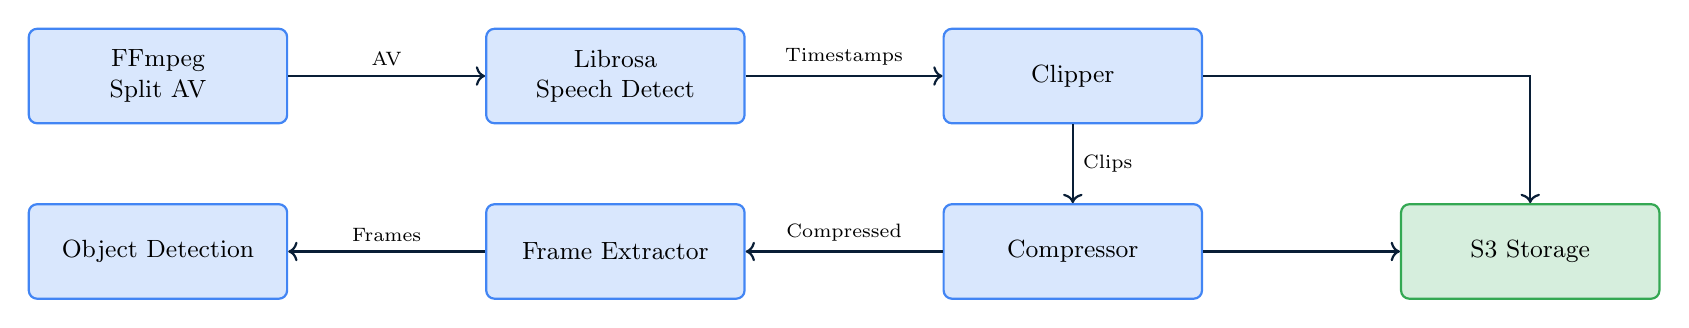
\begin{tikzpicture}[node distance=2.5cm]
        
        \node<1->[compute] (a) {FFmpeg\\Split AV};
        \node<2->[compute, right=of a] (b) {Librosa\\Speech Detect};
        \node<3->[compute, right=of b] (c) {Clipper};
        \node<4->[compute, below=1cm of c] (d) {Compressor};
        \node<5->[compute, left=of d] (e) {Frame Extractor};
        \node<6->[compute, left=of e] (f) {Object Detection};
        
        \node<7->[storage, right=of d] (s3) {S3 Storage};
        
        \draw<2->[arrow] (a) -- node[above]{\scriptsize AV} (b);
        \draw<3->[arrow] (b) -- node[above]{\scriptsize Timestamps} (c);
        \draw<4->[arrow] (c) -- node[right]{\scriptsize Clips} (d);
        \draw<5->[arrow] (d) -- node[above]{\scriptsize Compressed} (e);
        \draw<6->[arrow] (e) -- node[above]{\scriptsize Frames} (f);
        
        \draw<7->[arrow] (c) -| (s3);
        \draw<7->[arrow] (d) -- (s3);
        
        \end{tikzpicture}
        \end{adjustbox}
        \caption{Sequential and parallel pipeline stages execution.}
    \end{figure}
\end{frame}
\begin{frame}{Execution Flow}
    \begin{block}{How Data Moves Through the System}
        \begin{itemize}[<+->]
            \item The pipeline starts with a sequential flow:
            \begin{itemize}[<+->]
                \item ffmpeg $\rightarrow$ librosa $\rightarrow$ clipping $\rightarrow$ compression
            \end{itemize}
            \item After this point, the pipeline branches into two parallel paths:
            \begin{itemize}[<+->]
                \item One branch handles frame extraction and object detection
                \item The other handles audio processing and speech-to-text conversion
            \end{itemize}
            \item Managing this fan-out behavior was important to ensure correct scaling and data flow.
        \end{itemize}
    \end{block}
\end{frame}

\begin{frame}{Execution Flow: Fan-out Architecture}
    \vspace{0.3cm}
    \begin{figure}
        \centering
        \begin{adjustbox}{max size={0.8\textwidth}{0.7\textheight}}
        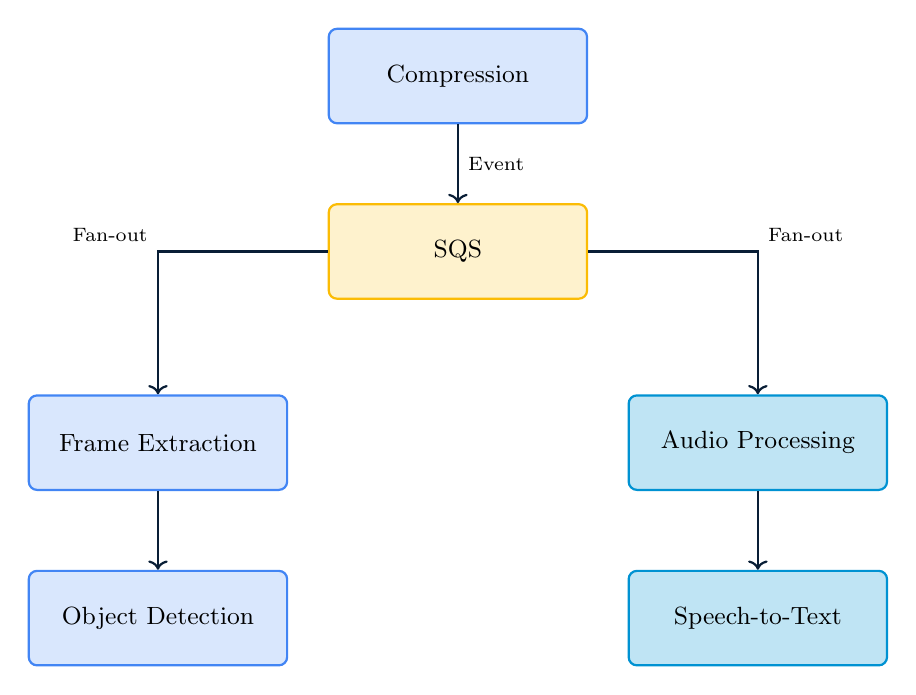
\begin{tikzpicture}[node distance=2.5cm]
        
        \node<1->[compute] (start) {Compression};
        
        \node<2->[queue, below=1cm of start] (q) {SQS};
        
        \node<3->[compute, below left=1.2cm and 0.5cm of q] (video) {Frame Extraction};
        \node<3->[compute, below right=1.2cm and 0.5cm of q, fill=OpenFaaSLight!25, draw=OpenFaaSLight] (audio) {Audio Processing};
        
        \node<4->[compute, below=1cm of video] (obj) {Object Detection};
        \node<4->[compute, below=1cm of audio, fill=OpenFaaSLight!25, draw=OpenFaaSLight] (speech) {Speech-to-Text};
        
        \draw<2->[arrow] (start) -- node[right]{\scriptsize Event} (q);
        
        \draw<3->[arrow] (q) -| node[above left]{\scriptsize Fan-out} (video);
        \draw<3->[arrow] (q) -| node[above right]{\scriptsize Fan-out} (audio);
        
        \draw<4->[arrow] (video) -- (obj);
        \draw<4->[arrow] (audio) -- (speech);
        
        \end{tikzpicture}
        \end{adjustbox}
        \caption{Fan-out topology routing multiple payloads synchronously.}
    \end{figure}
\end{frame}
\begin{frame}{Key Design Approach}
    \begin{block}{How I Approached the Problem}
        \begin{itemize}[<+->]
            \item Instead of rewriting the pipeline, I focused on adapting OpenFaaS to work with existing CLI-based scripts.
            \item I used the Classic Watchdog so that each function could run exactly like a normal terminal command.
            \item To handle missing dependencies, I created a lightweight stub package for \texttt{aisprint}.
            \item I also built wrapper scripts that convert HTTP requests into CLI arguments.
        \end{itemize}
    \end{block}
\end{frame}
\begin{frame}{Output Behavior}
    \begin{block}{Why Output Patterns Matter}
        \begin{itemize}[<+->]
            \item Some functions produce only a single output per request.
            \item However, stages like clip generation and frame extraction produce multiple outputs.
            \item This was important because it directly affected:
            \begin{itemize}[<+->]
                \item How I designed scaling
                \item And how I implemented queue-based fan-out execution
            \end{itemize}
        \end{itemize}
    \end{block}
\end{frame}
\begin{frame}{Enabling OpenFaaS: EKS Deployment}
    \begin{block}{Infrastructure Provisioning}
        \begin{itemize}[<+->]
            \item \textbf{EKS Cluster Creation}: Provisioned an Amazon Elastic Kubernetes Service (EKS) cluster utilizing managed node groups for dynamic auto-scaling.
            \item \textbf{OpenFaaS Helm Installation}: Deployed the OpenFaaS ecosystem into the cluster using standard Helm charts.
            \item \textbf{AWS ELB Exposure}: Created a NodePort/LoadBalancer service bridging internal Kubernetes networking to an Internet-facing AWS Elastic Load Balancer.
            \item \textbf{Deployment Pipelines}: Utilized \texttt{faas-cli deploy -f stack.yml} pointing perfectly to the remote ELB Gateway to construct and map Docker containers directly into EKS Pods.
        \end{itemize}
    \end{block}
\end{frame}

\begin{frame}{EKS Deployment: Topology}
    \vspace{0.3cm}
    \begin{figure}
        \centering
        \begin{adjustbox}{max size={\textwidth}{0.7\textheight}}
        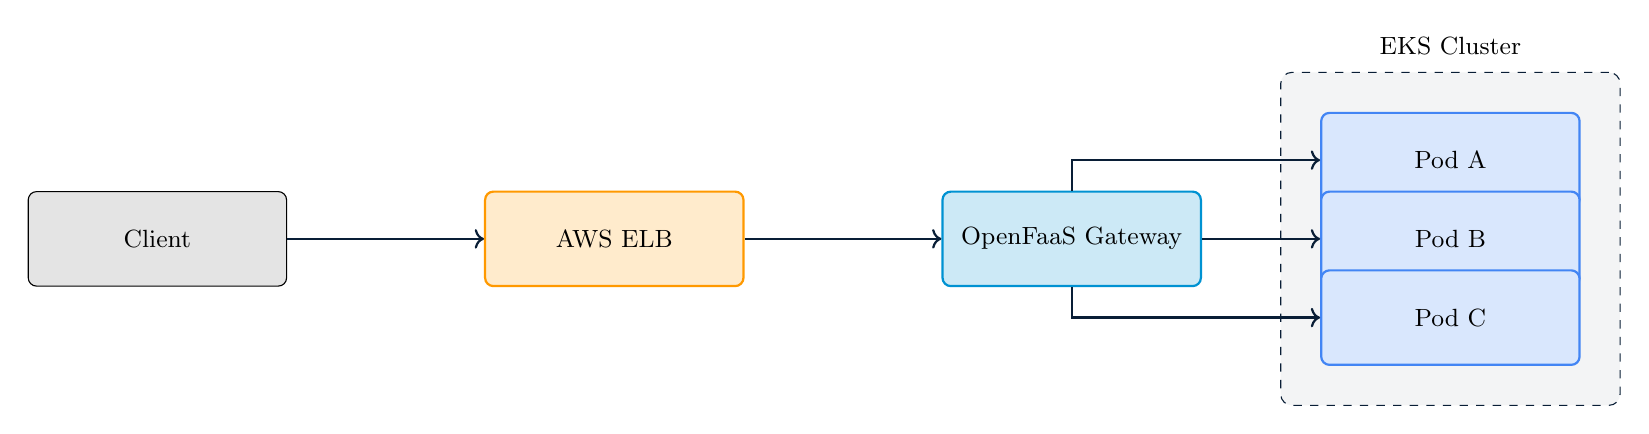
\begin{tikzpicture}[node distance=2.5cm]
        
        \node<1->[user] (user) {Client};
        \node<1->[aws, right=of user] (elb) {AWS ELB};
        \node<2->[gateway, right=of elb] (gateway) {OpenFaaS Gateway};
        
        \node<3->[compute, right=1.5cm of gateway, yshift=1cm] (pod1) {Pod A};
        \node<3->[compute, right=1.5cm of gateway] (pod2) {Pod B};
        \node<3->[compute, right=1.5cm of gateway, yshift=-1cm] (pod3) {Pod C};
        
        \begin{scope}[on background layer]
            \node<3->[draw=OpenFaaSDark, dashed, rounded corners, fill=OpenFaaSDark!5, fit={(pod1) (pod2) (pod3)}, inner sep=0.5cm] (cluster) {};
            \node<3-> at (cluster.north) [above=0.1cm] {\small EKS Cluster};
        \end{scope}
        
        \draw<1->[arrow] (user) -- (elb);
        \draw<2->[arrow] (elb) -- (gateway);
        \draw<3->[arrow] (gateway) |- (pod1);
        \draw<3->[arrow] (gateway) -- (pod2);
        \draw<3->[arrow] (gateway) |- (pod3);
        
        \end{tikzpicture}
        \end{adjustbox}
        \caption{AWS EKS physical deployment cluster outline.}
    \end{figure}
\end{frame}

\begin{frame}{Enabling OpenFaaS: Code Adaptation}
    \begin{block}{How I Made the Code Cloud-Ready}
        \begin{itemize}[<+->]
            \item Since the original scripts were not designed for serverless execution, I had to adapt them without modifying their logic.
            \item I used \texttt{fwatchdog} to convert HTTP requests into stdin/stdout-based execution.
            \item I removed dependency on local files by introducing S3-based input/output handling.
            \item All configuration was centralized into \texttt{stack.yml}, making deployment much cleaner.
        \end{itemize}
    \end{block}
\end{frame}

\begin{frame}{SQS-Based Orchestration}
    \begin{block}{Making the Pipeline Event-Driven}
        \begin{itemize}[<+->]
            \item Instead of manually triggering every stage, I used AWS SQS to connect all functions.
            \item Now, only the first function (\texttt{ffmpeg-0}) is triggered externally.
            \item Each function automatically triggers the next stage by sending a message to a queue.
            \item This made the system fully event-driven and much more scalable.
        \end{itemize}
    \end{block}
\end{frame}

\begin{frame}{SQS Orchestration: Flow Topology}
    \begin{figure}
        \centering
        \begin{adjustbox}{max size={\textwidth}{0.8\textheight}}
        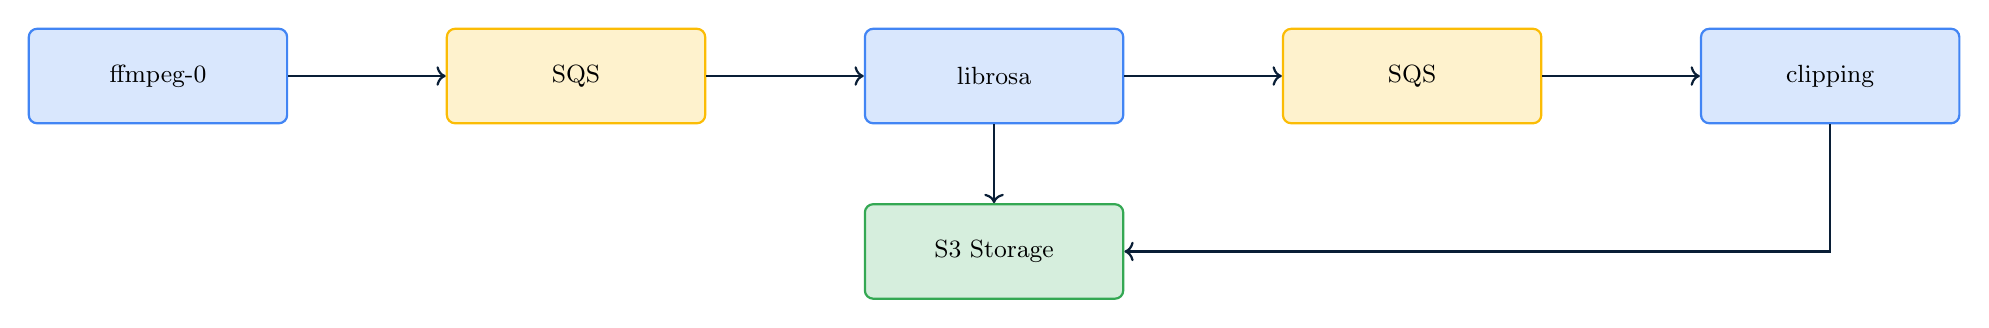
\begin{tikzpicture}[node distance=2cm]
        
        \node<1->[compute] (f1) {ffmpeg-0};
        
        \node<2->[queue, right=of f1] (q1) {SQS};
        \node<3->[compute, right=of q1] (f2) {librosa};
        
        \node<4->[queue, right=of f2] (q2) {SQS};
        \node<5->[compute, right=of q2] (f3) {clipping};
        
        \node<6->[storage, below=1cm of f2] (s3) {S3 Storage};
        
        \draw<2->[arrow] (f1) -- (q1);
        \draw<3->[arrow] (q1) -- (f2);
        \draw<4->[arrow] (f2) -- (q2);
        \draw<5->[arrow] (q2) -- (f3);
        
        \draw<6->[arrow] (f2) -- (s3);
        \draw<6->[arrow] (f3) |- (s3);
        
        \end{tikzpicture}
        \end{adjustbox}
        \caption{Event-driven AWS SQS integration linking pipeline stages.}
    \end{figure}
\end{frame}

\begin{frame}{End-to-End Architecture}
    \begin{figure}
        \centering
        \begin{adjustbox}{max size={0.9\textwidth}{0.8\textheight}}
        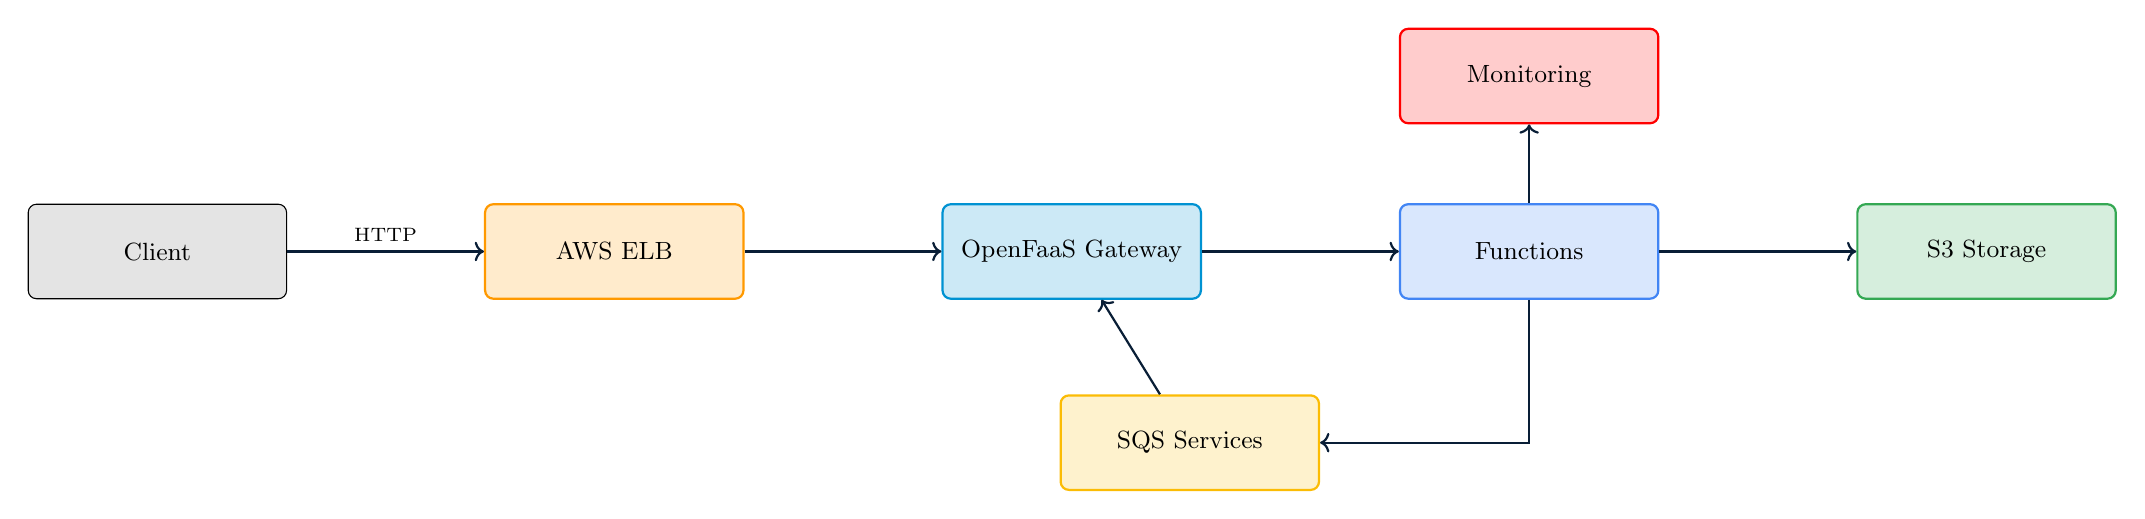
\begin{tikzpicture}[node distance=2.5cm]
        
        \node<1->[user] (user) {Client};
        \node<1->[aws, right=of user] (elb) {AWS ELB};
        \node<2->[gateway, right=of elb] (gateway) {OpenFaaS Gateway};
        
        \node<3->[compute, right=of gateway] (fn) {Functions};
        
        \node<4->[queue, below=1.2cm of gateway, xshift=1.5cm] (sqs) {SQS Services};
        \node<5->[storage, right=of fn] (s3) {S3 Storage};
        
        \node<6->[compute, above=1cm of fn, fill=red!20, draw=red] (monitor) {Monitoring};
        
        \draw<1->[arrow] (user) -- node[above]{\scriptsize HTTP} (elb);
        \draw<2->[arrow] (elb) -- (gateway);
        \draw<3->[arrow] (gateway) -- (fn);
        
        \draw<4->[arrow] (fn) |- (sqs);
        \draw<4->[arrow] (sqs) -- (gateway);
        
        \draw<5->[arrow] (fn) -- (s3);
        \draw<6->[arrow] (fn) -- (monitor);
        
        \end{tikzpicture}
        \end{adjustbox}
        \caption{End-to-end full serverless pipeline ecosystem view.}
    \end{figure}
\end{frame}


\begin{frame}{Logical System Architecture}
    \begin{figure}
        \centering
        \resizebox{\textwidth}{!}{
        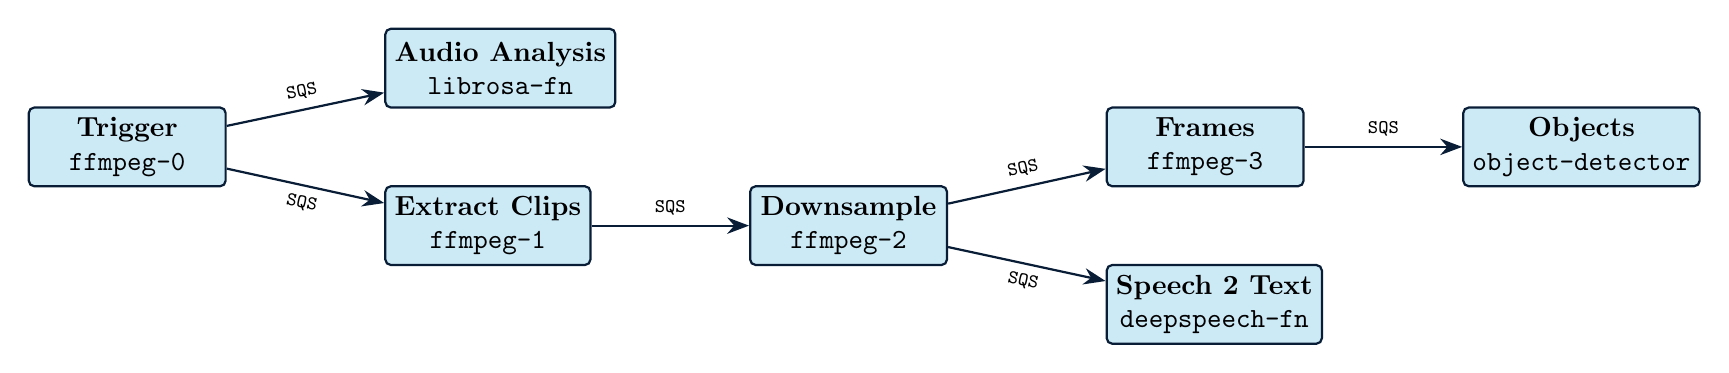
\begin{tikzpicture}[
            node distance=1.5cm and 2cm,
            box/.style={rectangle, draw=OpenFaaSDark, fill=OpenFaaSLight!20, thick, minimum width=2.5cm, minimum height=1cm, align=center, rounded corners=2pt},
            arrow/.style={-{Stealth[scale=1.2]}, thick, draw=OpenFaaSDark}
        ]
            % Nodes
            \node[box] (source) {\textbf{Trigger}\\ \texttt{ffmpeg-0}};
            \node[box, right=of source, yshift=1cm] (librosa) {\textbf{Audio Analysis}\\ \texttt{librosa-fn}};
            \node[box, right=of source, yshift=-1cm] (ff1) {\textbf{Extract Clips}\\ \texttt{ffmpeg-1}};
            \node[box, right=of ff1] (ff2) {\textbf{Downsample}\\ \texttt{ffmpeg-2}};
            \node[box, right=of ff2, yshift=1cm] (ff3) {\textbf{Frames}\\ \texttt{ffmpeg-3}};
            \node[box, right=of ff3] (yolo) {\textbf{Objects}\\ \texttt{object-detector}};
            \node[box, right=of ff2, yshift=-1cm] (ds) {\textbf{Speech 2 Text}\\ \texttt{deepspeech-fn}};

            % Arrows
            \draw[arrow] (source) -- node[above, sloped] {\scriptsize \texttt{SQS}} (librosa);
            \draw[arrow] (source) -- node[below, sloped] {\scriptsize \texttt{SQS}} (ff1);
            \draw[arrow] (ff1) -- node[above] {\scriptsize \texttt{SQS}} (ff2);
            \draw[arrow] (ff2) -- node[above, sloped] {\scriptsize \texttt{SQS}} (ff3);
            \draw[arrow] (ff2) -- node[below, sloped] {\scriptsize \texttt{SQS}} (ds);
            \draw[arrow] (ff3) -- node[above] {\scriptsize \texttt{SQS}} (yolo);
        \end{tikzpicture}
        }
        \caption{Event-driven OpenFaaS pipeline reliant on S3 mapped payloads.}
    \end{figure}
    
\end{frame}

\begin{frame}{Key Fixes and Improvements}
    \begin{block}{Major Issues I Solved}
        \begin{itemize}[<+->]
            \item I implemented Locust alongside JMeter to compare performance under different load models.
            \item Fixed a critical concurrency issue where multiple requests were overwriting data in \texttt{/tmp}.
            \item Solved S3 data loss problems by ensuring unique output paths for each invocation.
            \item Improved queue routing logic so that fan-out stages correctly propagate data downstream.
        \end{itemize}
    \end{block}
    \begin{figure}
        \centering
        \begin{adjustbox}{max size={0.8\textwidth}{0.8\textheight}}
        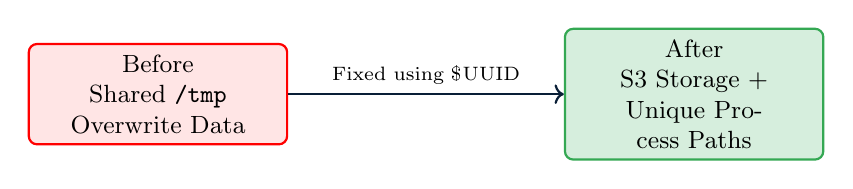
\begin{tikzpicture}[node distance=3.5cm]
        
        \node[compute, fill=red!10, draw=red] (before) {Before\\Shared \texttt{/tmp}\\Overwrite Data};
        
        \node[storage, right=of before] (after) {After\\S3 Storage +\\Unique Process Paths};
        
        \draw[arrow, thick] (before) -- node[above]{\scriptsize Fixed using \$UUID} (after);
        
        \end{tikzpicture}
        \end{adjustbox}
        \caption{Fixing data overwrites using S3 URIs across parallel invocations.}
    \end{figure}
\end{frame}

\begin{frame}{Visual Architecture: Load Testing}
    \begin{figure}
        \centering
        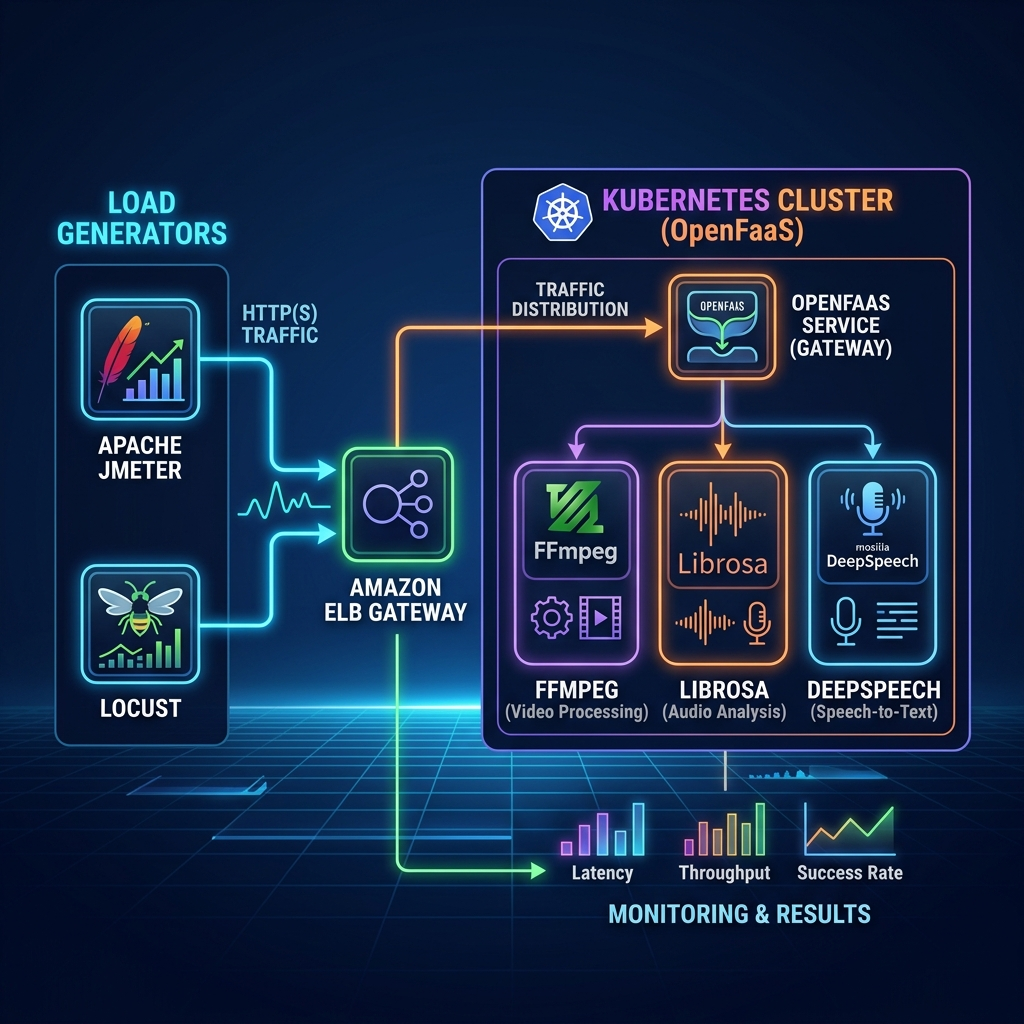
\includegraphics[width=0.85\textwidth,height=0.7\textheight,keepaspectratio]{images/architecture.png}
        \caption{Load Testing Architecture Layout.}
    \end{figure}
\end{frame}

\begin{frame}{Testing Methodology}
    We simulated user-workloads sending requests to the system utilizing two different load generation mechanisms: \textbf{Apache JMeter} and \textbf{Locust}.
    \vspace{0.2cm}
    
    \begin{exampleblock}{Test Configuration Pipeline}
        \begin{itemize}[<+->]
            \item \textbf{Target Endpoint}: \texttt{/function/ffmpeg-0} gateway instance
            \item \textbf{Concurrency Levels}: 5, 10, and 15 simulated users
            \item \textbf{Think Time}: 20 seconds exponential backoff
            \item \textbf{Duration}: 5 minutes (300 seconds) per tier
            \item \textbf{Ramp-up}: 10 seconds duration
        \end{itemize}
    \end{exampleblock}
\end{frame}

\begin{frame}{Results: Apache JMeter}
    \begin{columns}
        \begin{column}{0.48\textwidth}
            \begin{table}[]
                \centering
                \renewcommand{\arraystretch}{1.2}
                \resizebox{\textwidth}{!}{
                \begin{tabular}{l c c c l}
                    \toprule
                    \textbf{Users} & \textbf{Runs} & \textbf{Avg (ms)} & \textbf{Max (ms)} & \textbf{Fail} \\
                    \midrule
                    5   & 76  & 1708 & 2273 & 0\% \\
                    10  & 143 & 1837 & 3297 & 0\% \\
                    15  & 200 & 2325 & 5147 & 0\% \\
                    \bottomrule
                \end{tabular}}
                \caption{JMeter execution metrics.}
            \end{table}
            \vspace{0.2cm}
            \begin{itemize}[<+->]
                \item Handled continuous scale perfectly without degradation.
                \item Response time rose 36\% under peak simulated load.
            \end{itemize}
        \end{column}
        \begin{column}{0.48\textwidth}
            \begin{figure}
                \centering
                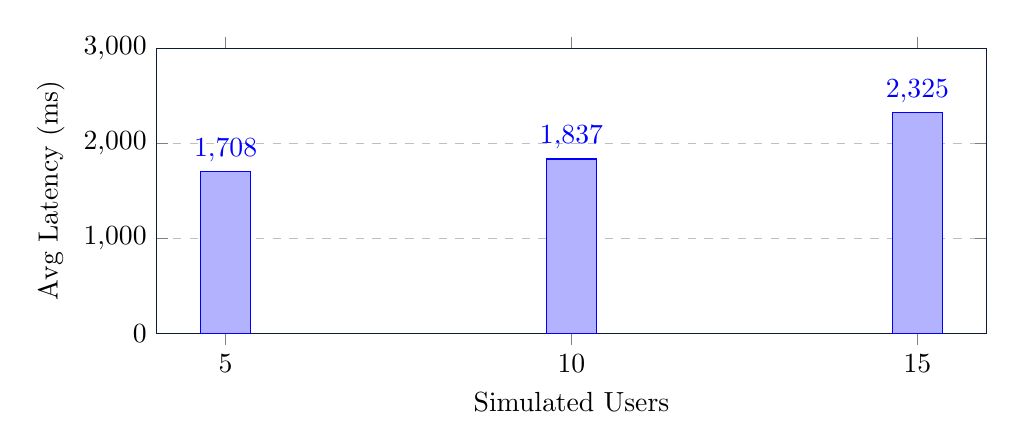
\begin{tikzpicture}
                    \begin{axis}[
                        ybar,
                        bar width=18pt,
                        width=\textwidth,
                        height=5.2cm,
                        xlabel={Simulated Users},
                        ylabel={Avg Latency (ms)},
                        symbolic x coords={5, 10, 15},
                        xtick=data,
                        nodes near coords,
                        nodes near coords align={vertical},
                        ymin=0, ymax=3000,
                        ymajorgrids=true,
                        grid style=dashed,
                        fill=OpenFaaSLight,
                        draw=OpenFaaSDark
                    ]
                    \addplot coordinates {(5,1708) (10,1837) (15,2325)};
                    \end{axis}
                \end{tikzpicture}
                \caption{JMeter Latency trend.}
            \end{figure}
        \end{column}
    \end{columns}
\end{frame}

\begin{frame}{Results: Locust Framework}
    \begin{columns}
        \begin{column}{0.48\textwidth}
            \begin{table}[]
                \centering
                \renewcommand{\arraystretch}{1.2}
                \resizebox{\textwidth}{!}{
                \begin{tabular}{l c c c l}
                    \toprule
                    \textbf{Users} & \textbf{Runs} & \textbf{Avg (ms)} & \textbf{Max (ms)} & \textbf{Fail} \\
                    \midrule
                    5   & 78  & 1717 & 3505 & 0 \\
                    10  & 145 & 2046 & 6008 & 1 \\
                    15  & 136 & 2980 & 9153 & 0 \\
                    \bottomrule
                \end{tabular}}
                \caption{Locust metrics.}
            \end{table}
            \vspace{0.2cm}
            \begin{itemize}[<+->]
                \item Python-based model logged higher tail latency.
                \item Single failure detected ($<1\%$) under peak load.
            \end{itemize}
        \end{column}
        \begin{column}{0.48\textwidth}
            \begin{figure}
                \centering
                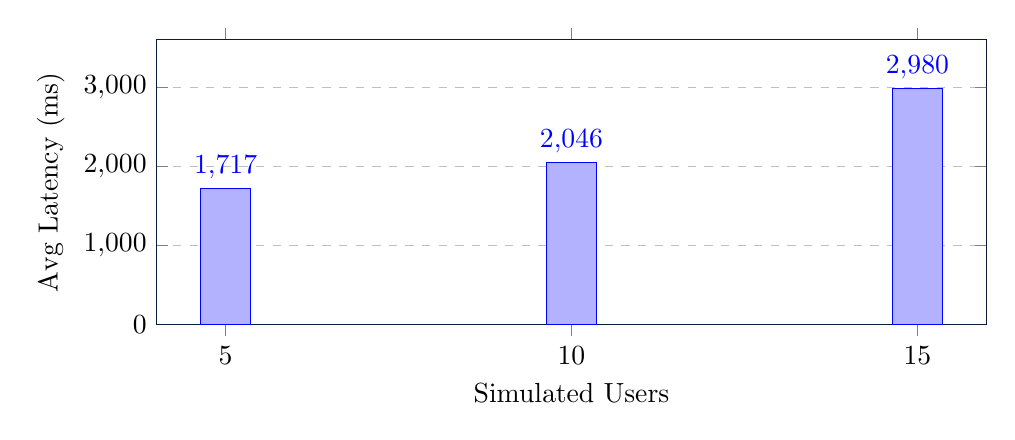
\begin{tikzpicture}
                    \begin{axis}[
                        ybar,
                        bar width=18pt,
                        width=\textwidth,
                        height=5.2cm,
                        xlabel={Simulated Users},
                        ylabel={Avg Latency (ms)},
                        symbolic x coords={5, 10, 15},
                        xtick=data,
                        nodes near coords,
                        nodes near coords align={vertical},
                        ymin=0, ymax=3600,
                        ymajorgrids=true,
                        grid style=dashed,
                        fill=OpenFaaSLight,
                        draw=OpenFaaSDark
                    ]
                    \addplot coordinates {(5,1717) (10,2046) (15,2980)};
                    \end{axis}
                \end{tikzpicture}
                \caption{Locust Latency trend.}
            \end{figure}
        \end{column}
    \end{columns}
\end{frame}

\begin{frame}{Summary \& Conclusions}
    \begin{itemize}[<+->]
        \item \textbf{Reliability:} The system achieved a stable execution with nearly 99.9\% success rate under continuous load.
        \item \textbf{Scalability:} The pipeline handled increasing users smoothly with only moderate latency increase.
        \item \textbf{Key Achievement:} I was able to convert a CLI-based pipeline into a fully serverless, event-driven system without modifying the original code.
        \item \textbf{Learning:} This project helped me understand real-world challenges like distributed execution, concurrency issues, and cloud deployment.
    \end{itemize}
\end{frame}

\end{document}
